%  !TEX root = ../main.tex


\subsection{Ultrasonic Adversarial Perturbation Delivery}\label{sec:preliminary_uap_delivery}
% 感觉这里需要体现出无声攻击的工作pipeline, 这样的话更容易让人理解
We envision that the above failure can be addressed by leveraging the vulnerability of ASR models to craft universal adversarial perturbations. Notably, it is promising to deliver the perturbation in an ultrasound-based manner to eventually reach the goal, i.e., the adversary can alter any user commands into a targeted one while guaranteeing entirely inaudible to the victim. However, we find the well-trained perturbations that are effective in digital domain all fail after being directly modulated and emitted by the ultrasound-based attack method (results are also given in \textsection\ref{sec:eval_utm}, \textit{G2}). 

Since the ultrasonic channel is lossy and distorted, to obtain a perturbation that can still effectively tamper with user commands after a series of processing based on ultrasound-based attack mechanisms and over-the-air delivery, i.e., the pipeline shown in Fig.~\ref{fig:dolphinattack_pipeline}, we need to precisely model the transformation from a perturbation in the digital domain to its physical version.
However, generalizing an AE from the digital to the physical world is inherently difficult, which has been proved by substantial research in both computer vision and audio community~\cite{jan2019connecting,carlini2018audio,chen2020metamorph,schonherr2020imperio,li2020advpulse,deng2022fencesitter,guo2022specpatch}. 
This issue in the audio domain refers to the fact that played-out speech samples are subject to signal distortion and environment interference (i.e., reverberation, attenuation, and noises). 
Previous audible-band works~\cite{rirIJCAI,schonherr2020imperio} have paid efforts in simulating the physical world by adopting room impulse response (RIR) during the AE optimization process to close the gap between the digital and physical world. Moreover, no work has yet been proposed on modeling ultrasonic delivery.
We are motivated to investigate the feasibility of applying audible-band modeling technologies to our unique ultrasonic case.
% ----------------------------- 2023.1.16 以上内容凝练之后整理到Sec 3.3中 -----------------------------
\begin{figure}[t]
    \centering
    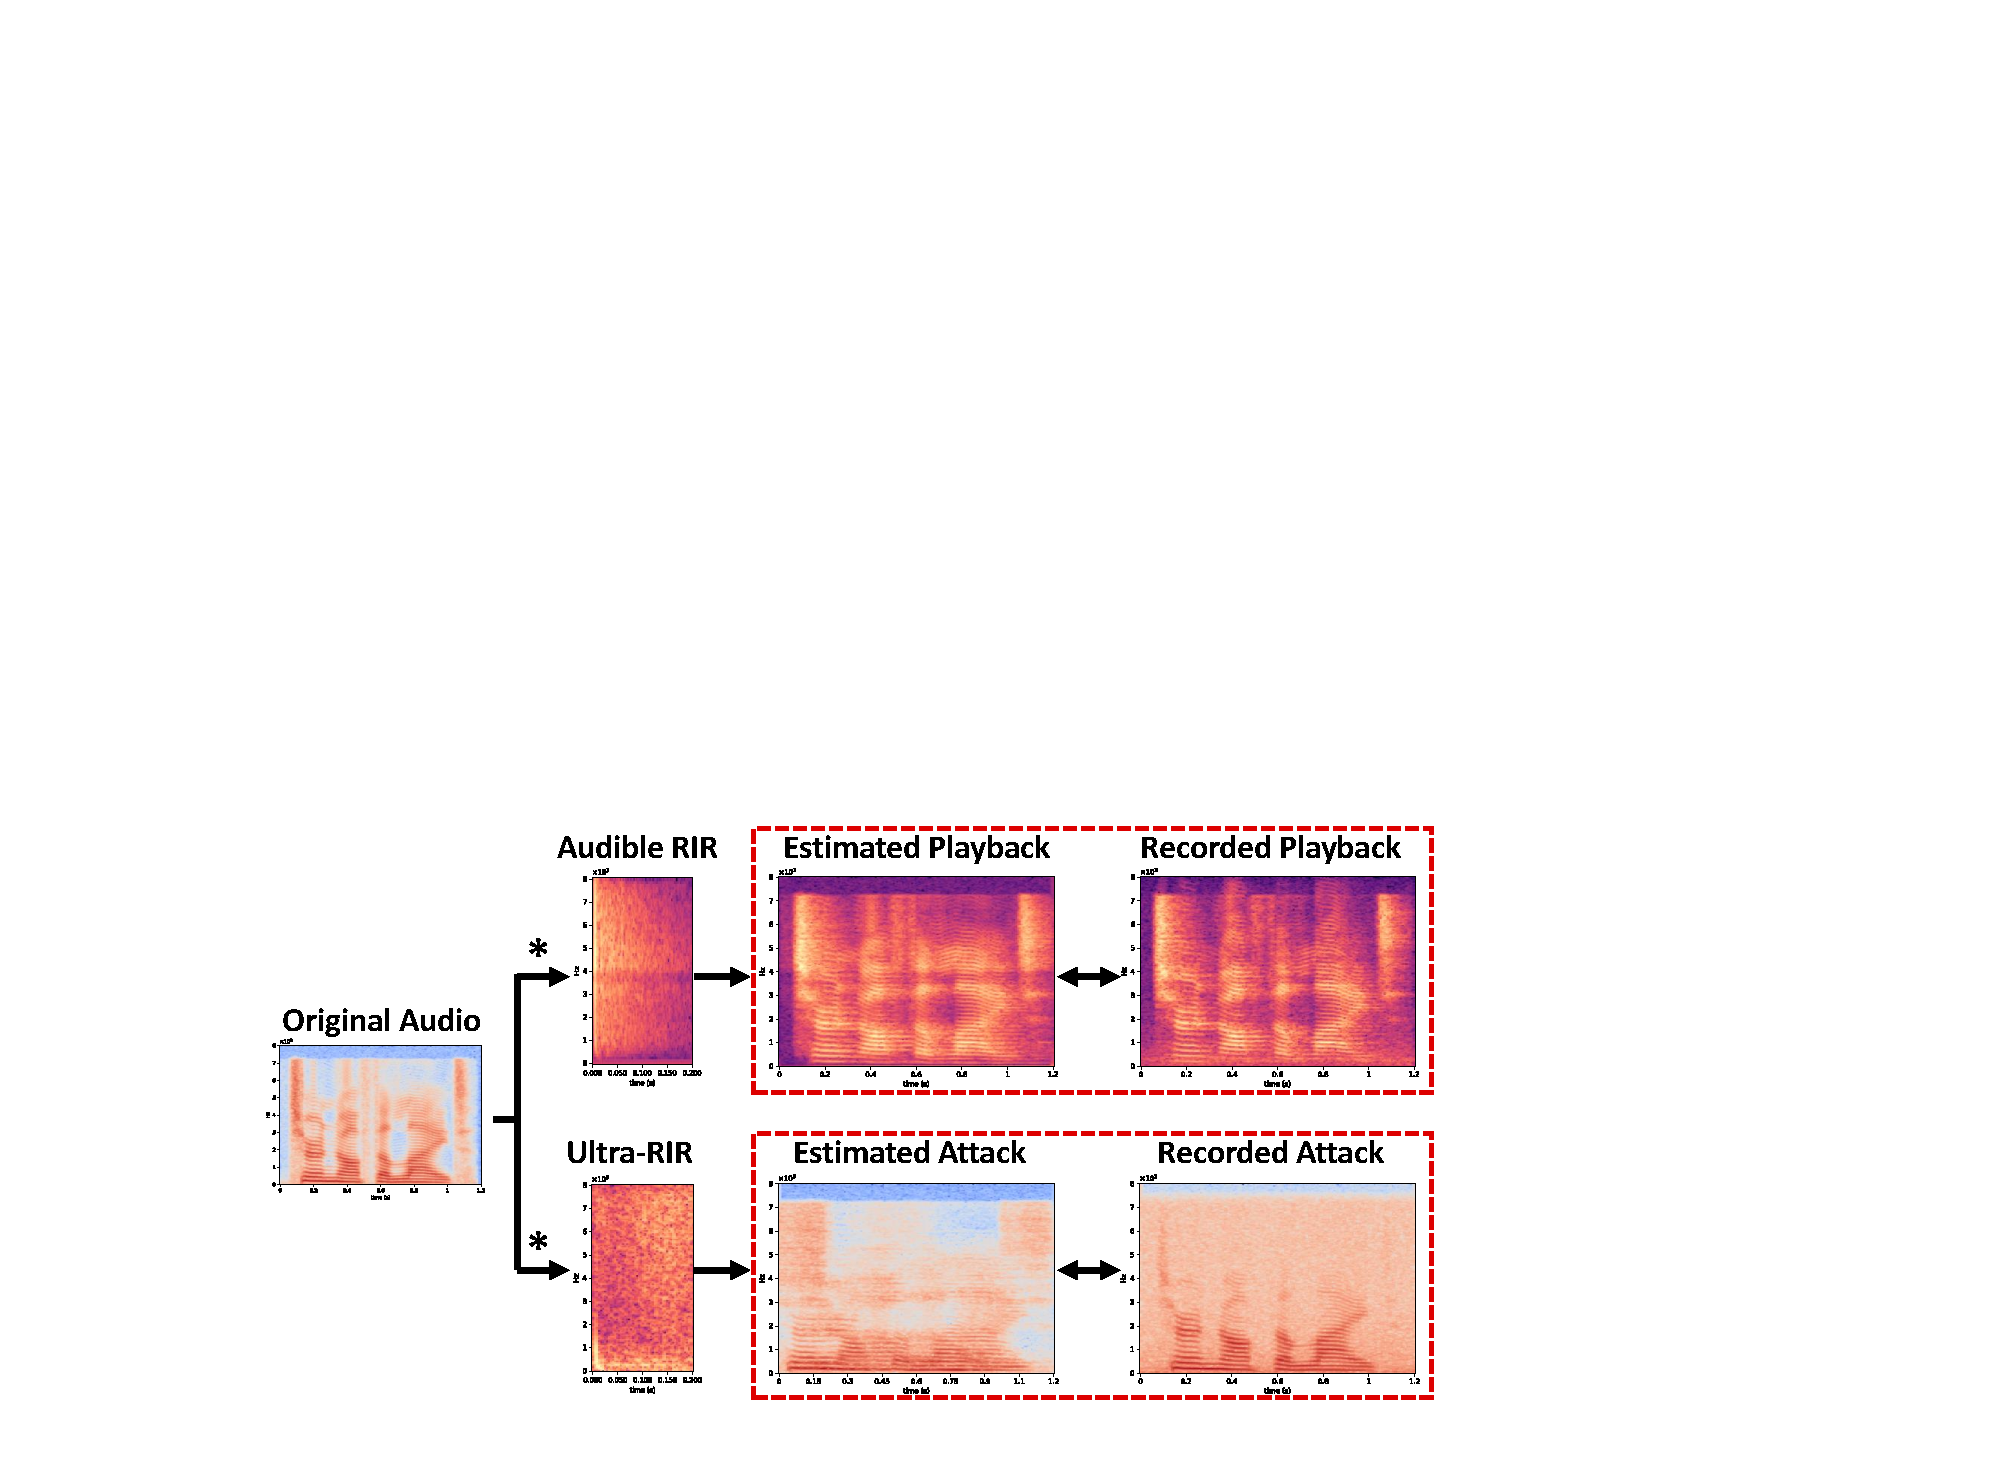
\includegraphics[width=0.35\textwidth]{est_actual_via_ir2.pdf}
    \caption{\label{fig:est_rir}Comparison between the audible RIR and ultra-RIR in estimating the digital-to-physical transformation.}
    \vspace{-10pt}
\end{figure}
\subsection{Attempts at Ultrasound Delivery Modeling}
In this subsection, we elaborate on applying two potentially feasible modeling methods for our case.

\subsubsection{Modeled by room impulse response}\label{sec:classic_rir}
Inspired by the success of audible-band AEs~\cite{rirIJCAI,schonherr2020imperio} drawing on the ability of RIR, which describes the reverberation and attenuation during audible sound propagation, we envisage that a similar RIR idea can generalize to characterize the ultrasound transformation process. Specifically, they exploit existing RIR databases~\cite{jeub2009binaural,nakamura2000acoustical} by convolving random RIR clips with digital adversarial signals in the optimization process, simulating the audio recorded by the receiver in various scenes, e.g., large concert hall and narrow corridor.
Therefore, we modulate the ideal impulse signal as the baseband on an ultrasound carrier and receive it on the recording device. With the obtained ``ultra-RIR'', we perform convolution with the original audio, whose output are expected to well represent the actually demodulated inaudible attack's result. As a comparison, we also conduct similar operations via a JBL loudspeaker for audible audio.
Fig.~\ref{fig:est_rir} shows that the estimated audible audio with RIR is very close to the actual playback. However, for the inaudible aspect, there is significant gap between the recorded attack audio and the estimated using ultra-RIR.
We believe the reason for such a mismatch is that the RIR rationale relies on the linear time-invariant (LTI) system prerequisite. However, the transformation is nonlinear because ultrasound-based attacks leverage microphones' nonlinearity vulnerability. % of ultrasound-based attacks leverages , i.e., the transformation is essentially nonlinear as shown in Eq.~\ref{equ:nonlinearity} where exponent terms exist. 


\begin{figure}[t]
    \centering
    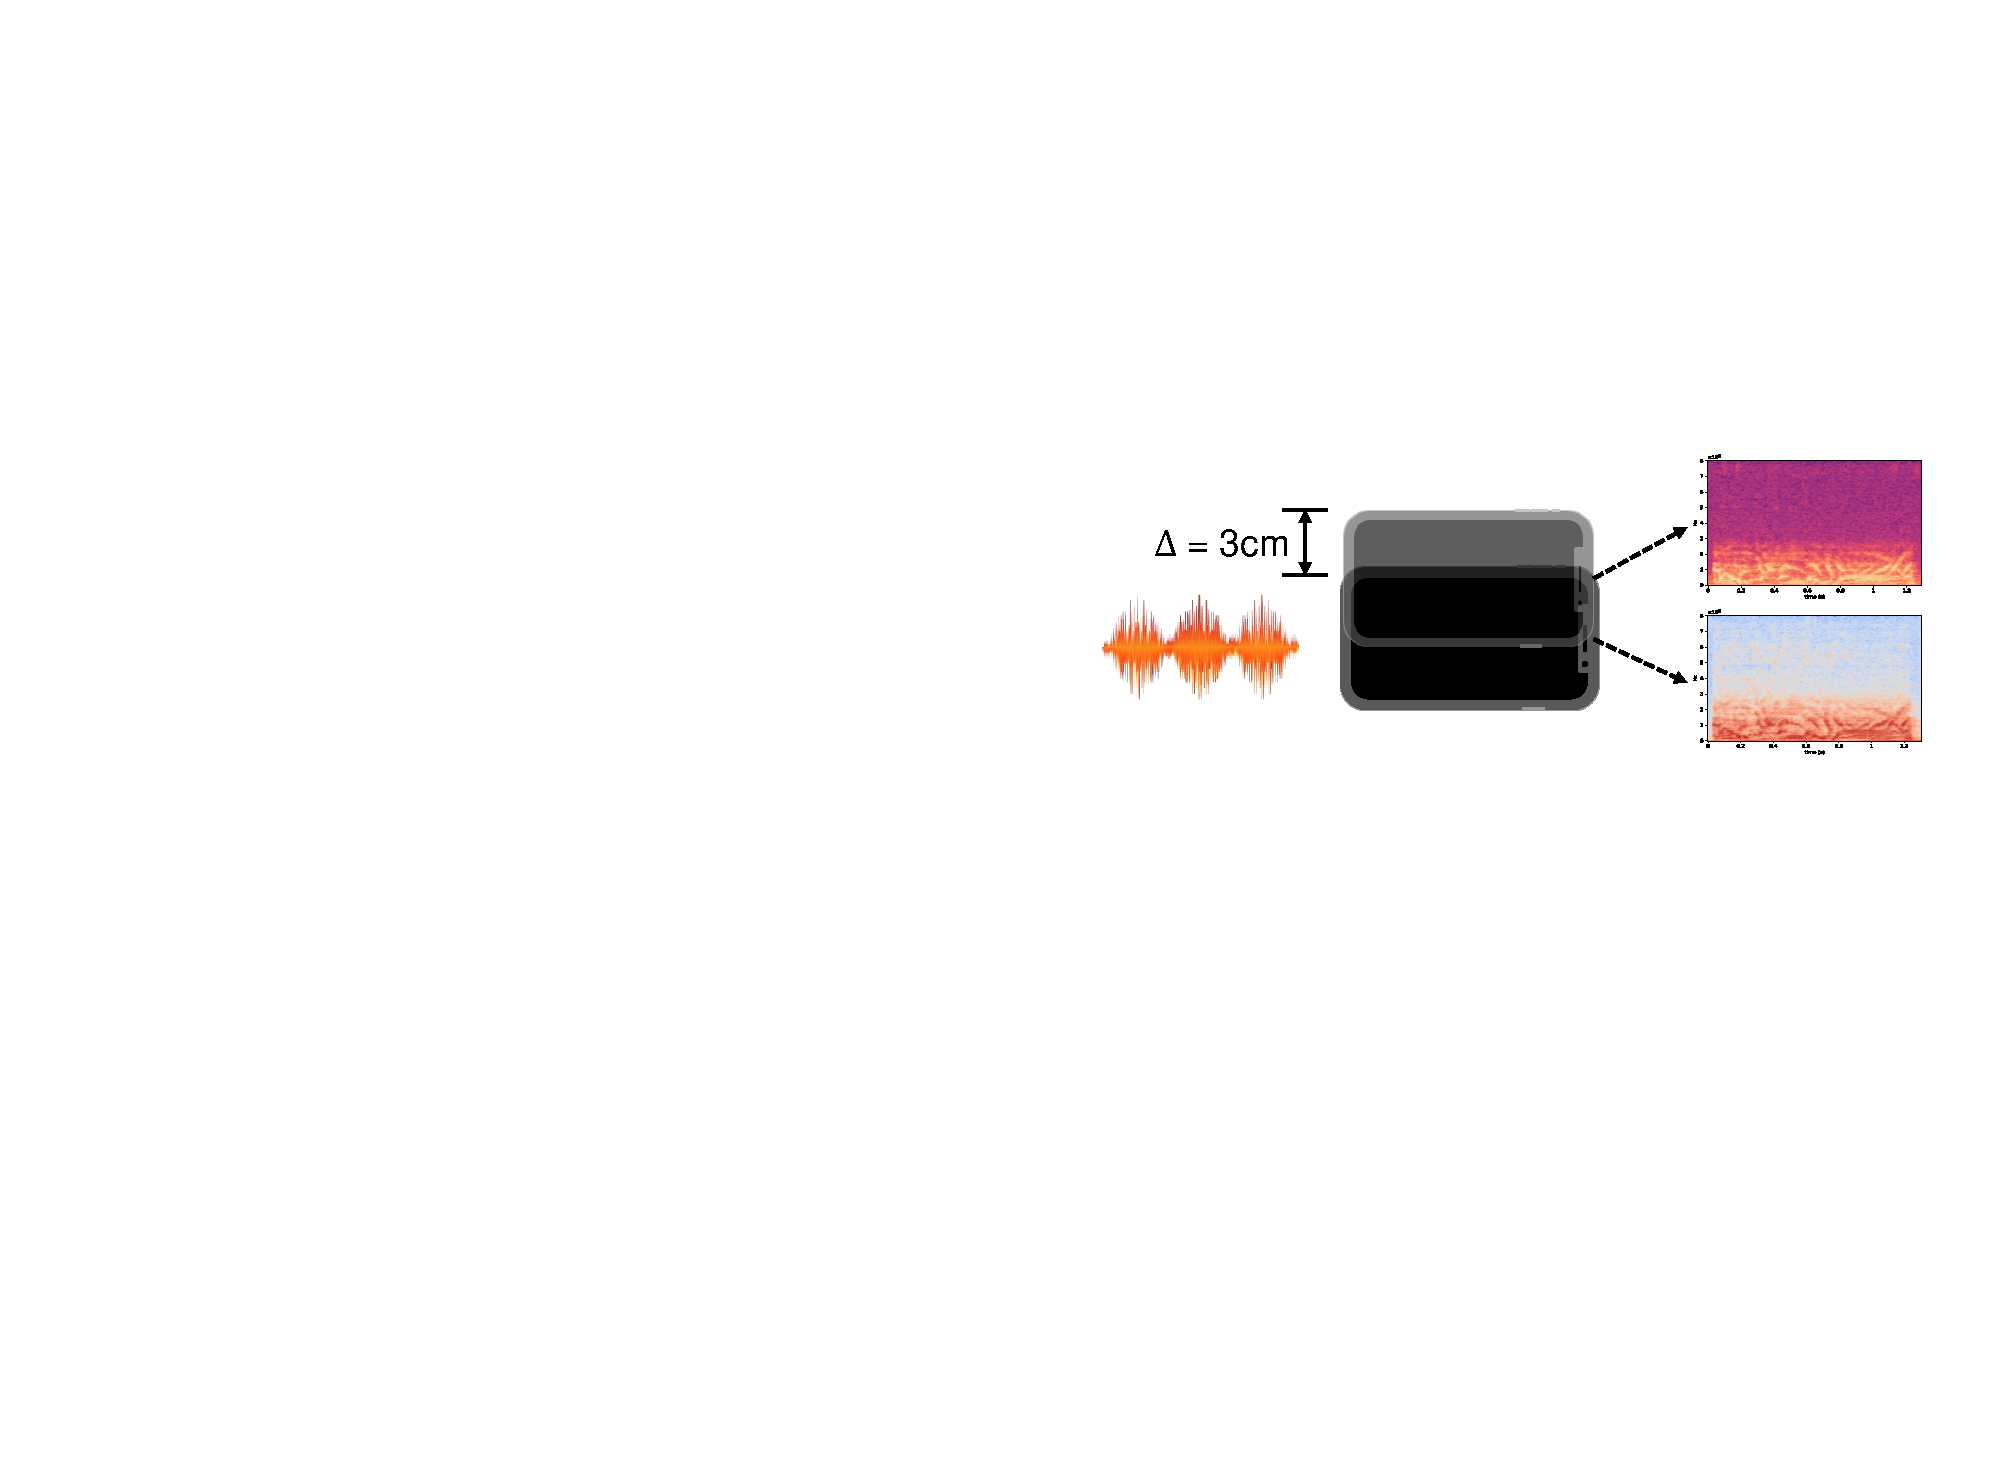
\includegraphics[width=0.3\textwidth]{AE_sensitivity2.pdf}
    \caption{\label{fig:AE_sensitivity}Illustration of displacement-induced changes in recorded audio.}
    \vspace{-10pt}
\end{figure}

\subsubsection{Modeled by Neural Network}\label{sec:classic_nn}
Since RIR is originally designed for LTI systems, neural networks with excellent nonlinear fitting capability should work well given their success in various tasks, e.g., speech denosing~\cite{hu2020dccrn} and image printing distortion~\cite{jan2019connecting}. 
Considering that an adversary expects a practical transformation model with minimal effort (i.e., dataset requirements) while guaranteeing its generality, we implement a multi-layer perception model (MLP) with only 60k parameters, using 120-second aligned original and ultrasound-based attack audio pairs. We find that the MLP can achieve a generalized capability of mapping digital-to-physical world spectrums between unseen pairs, but with position-dependent constraints. As shown in Fig.~\ref{fig:AE_sensitivity}, a slight position displacement (3~cm) leads to an apparent change (i.e. bringing anomalous noises) in the recovered baseband, which can cause the trained network to fail to estimate the recorded audio at various positions. 
Overall, although MLP builds a functional mapping for the nonlinear ultrasound transformation in a fixed relative position, it is too restricted due to the nature of ultrasound (cf. \textsection\ref{sec:ultrasound_observation}). Besides, adopting distance $d$ and angle $\theta$ as conditional network parameters might help, but collecting data for each position is endless.



\begin{figure}[t]
    \centering
    % \includegraphics[width=0.22\textwidth]{ultra25kvs1k-v3.pdf}
    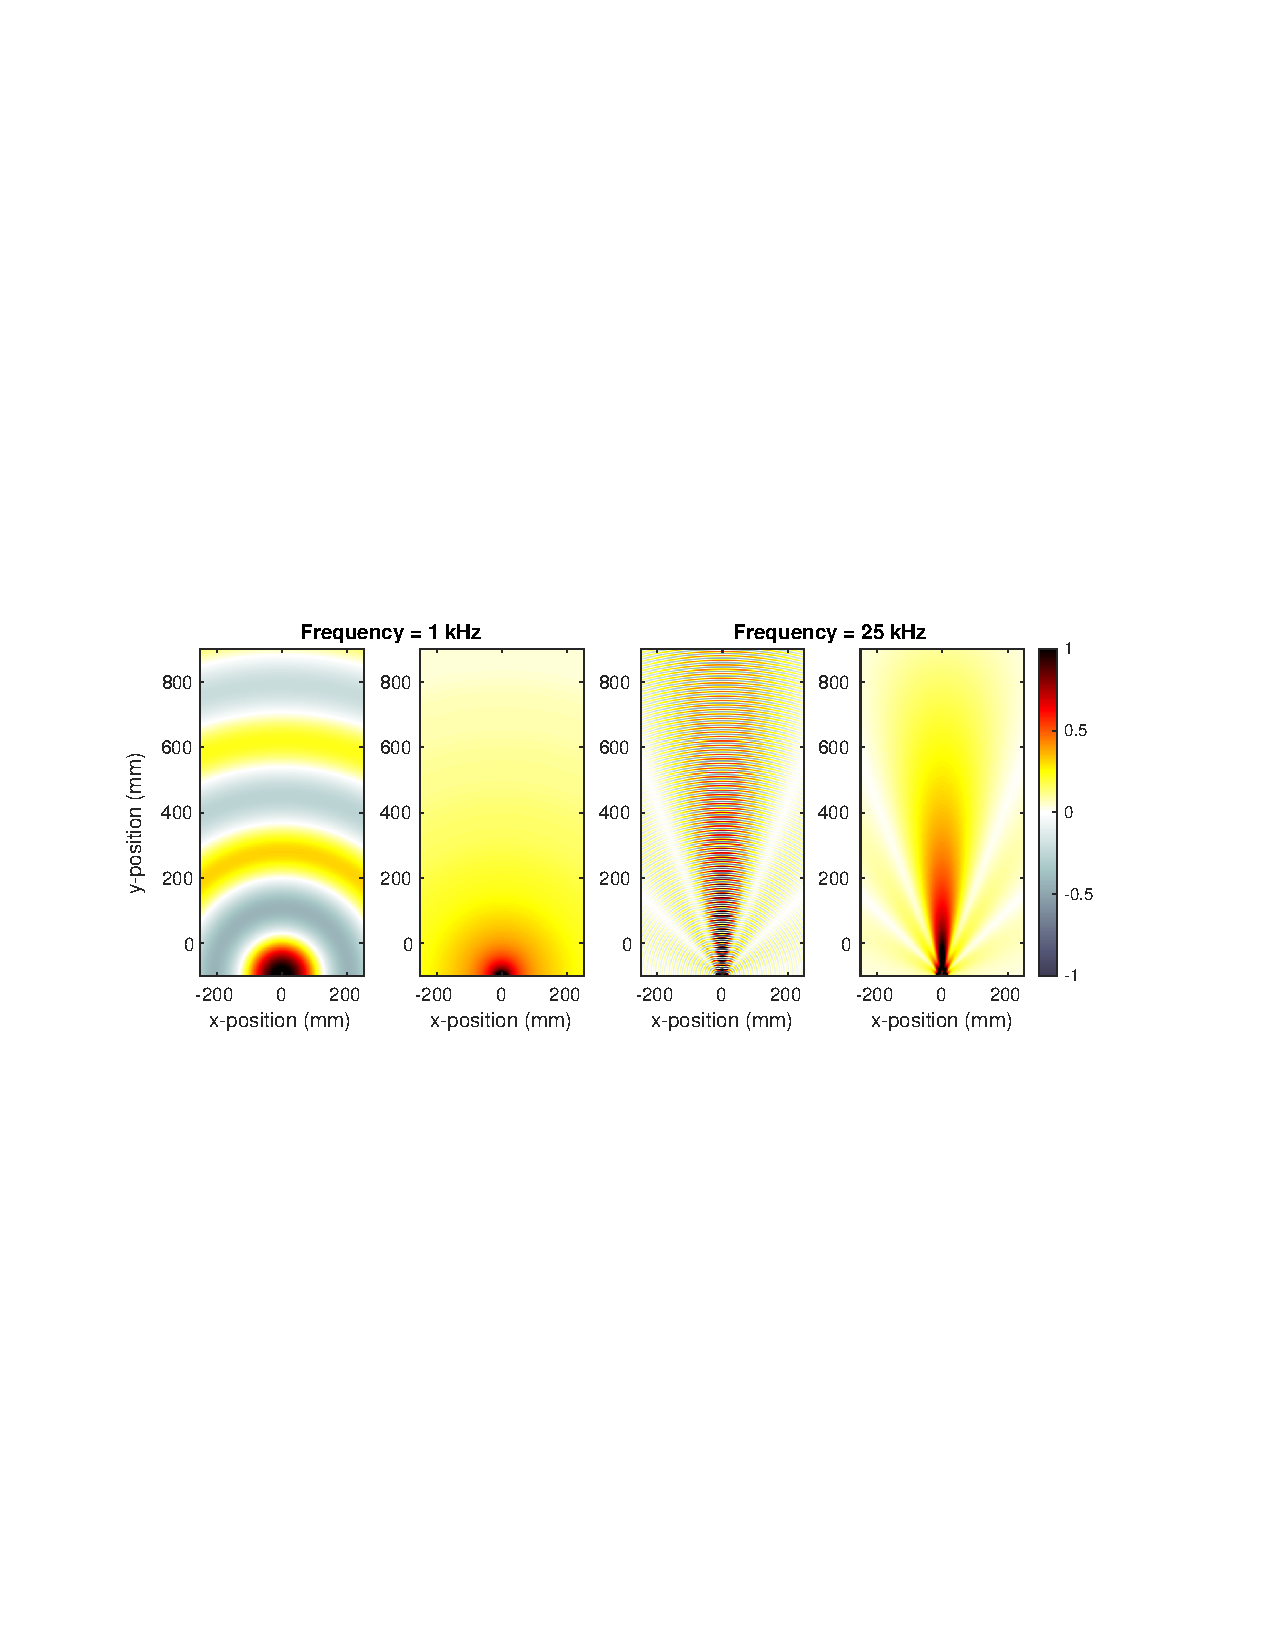
\includegraphics[width=0.36\textwidth]{ultrasound_field_press_sqrt2.pdf}
    \caption{\label{fig:soundfield}2-D sound fields simulation for comparing the audible wave with ultrasound.}
    \vspace{-15pt}
\end{figure}

\begin{figure*}[!t]
    \centering
    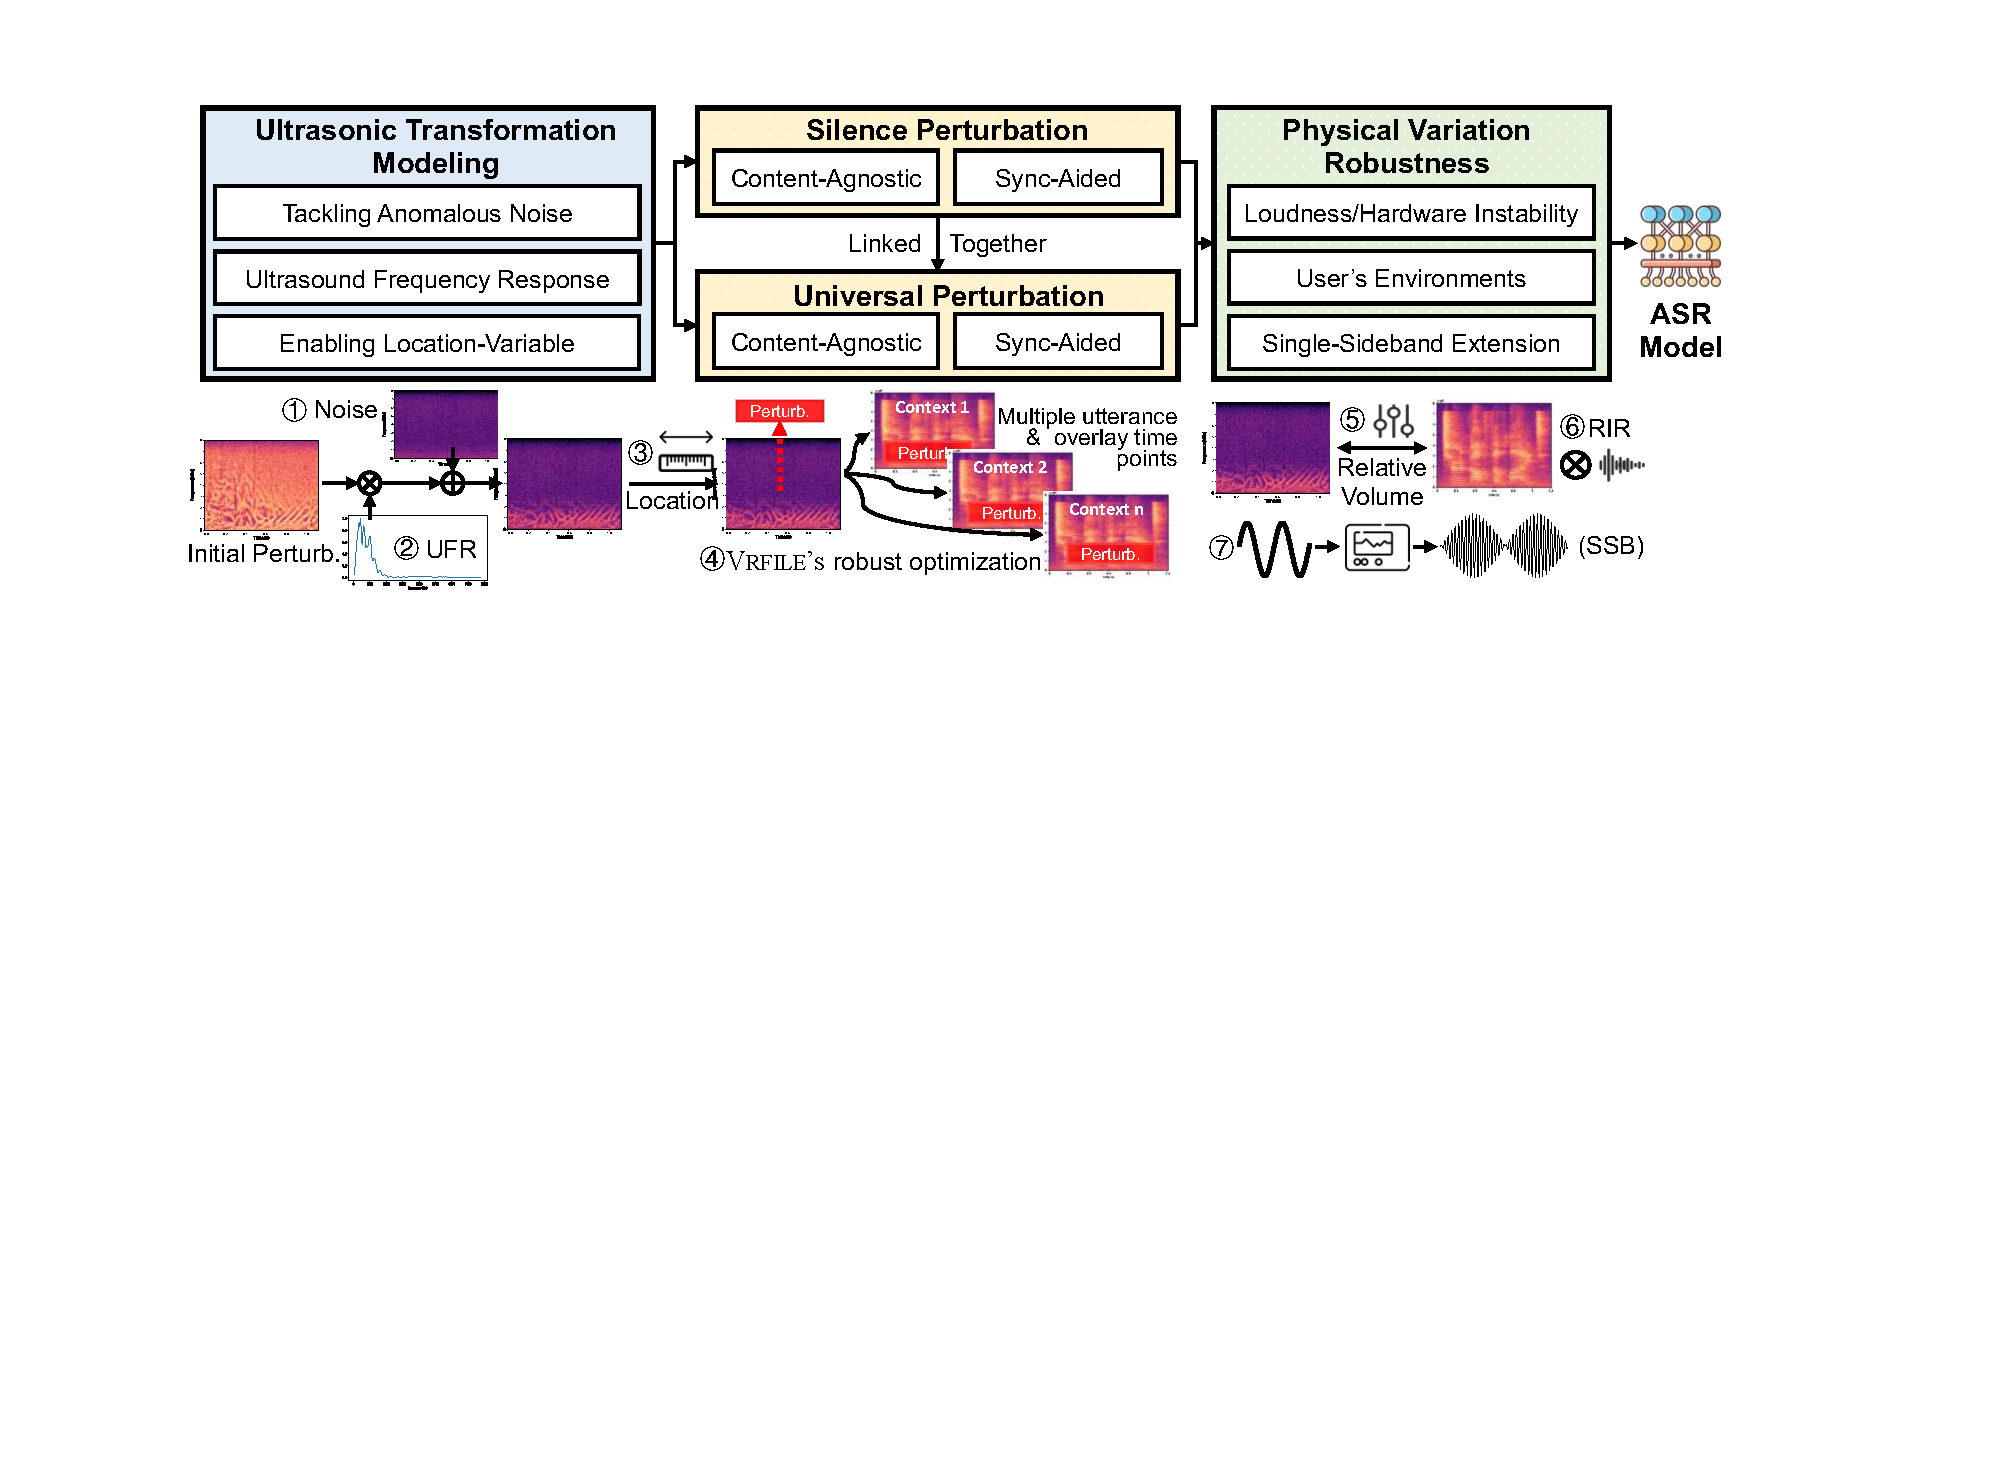
\includegraphics[width=0.95\textwidth]{design_overview4.pdf}
    \caption{Workflow of \alias. \ding{172}-\ding{174}: the ultrasonic transformation precisely describes the perturbation changes during physical delivery. \ding{175}: the transformed perturbation is involved into optimization for silence and universal attack purpose. \ding{176}-\ding{178}: we boost the attack's physical-world robustness from multiple aspects.}
    \label{fig:design_overview}
    \vspace{-15pt}
\end{figure*}


\subsection{Challenges in Ultrasonic Delivery Modeling}\label{sec:ultrasound_observation}
The above attempts' failure drives us to look into the root cause of why modeling ultrasonic transformation is challenging. Ultrasound is intrinsically distinct from audible sounds due to its much higher frequency, and ultrasonic delivery leverages microphones' nonlinearity.
We also summarize the following characteristics:\\ % 或者说为何如此特殊
\begin{itemize}[leftmargin=*,topsep=-20pt]
    \item \emph{Ultrasound-induced Noise:} % \item \emph{Unpredictable Anomalous Noise:}
    The ultrasound carrier continuously forces the diaphragm to vibrate, probably resulting in anomalous noise in recorded attack alike Fig.~\ref{fig:est_rir}\&\ref{fig:AE_sensitivity}. Combined with such variable ultrasound fields, a slight displacement (e.g., 3~cm) can lead to different audio patterns.
    \item \emph{Nonlinear Distortion:} Eq.~\ref{equ:nonlinearity} indicates the I/O relationship of nonlinear demodulation, in which the factors $k_i$ is unknown and varies with recording devices~\cite{li2023learning}. 
    \item \emph{Varying Soundfield:} As shown in Fig.~\ref{fig:soundfield}, ultrasound field (25~kHz) is significantly more directional and changes more dramatically than audible waves (1~kHz) due to the much shorter wavelength.
    \item \emph{Hardware-induced Instability:} Ultrasound-based attacks rely on a series of signal processing and sophisticated devices, thus bringing instability due to hardware imperfection. 
\end{itemize}



\iffalse
\subsection{Challenges in Ultrasonic Transformation}\label{ultra_challenges}
The above attempts' failure drove us to look into the root cause why modeling ultrasonic transformation is challenging. In addition to the nonlinear distortion and anomalous noise problems revealed above, we also find the following characteristics:\\ % 或者说为何如此特殊
\textbf{Dramatically Changing Ultrasound Field:}\label{ultra_challenges:soundfield}
We employ the k-Wave toolbox~\cite{treeby2010k} to visually render the ultrasonic and audible sound fields in Fig.~\ref{fig:soundfield}, where the 1~kHz audible field is uniform and smooth. By contrast, the 25~kHz ultrasound field is significantly more directional and changes more dramatically because of the much shorter wavelength. Therefore, it casts great challenges to implement a location-agnostic attack as the audible-band attacks can do, as shown in Fig.~\ref{fig:AE_sensitivity}, where the slight position shift will lead to different transformations. Another phenomenon resulting from this drastic change is that the ultrasound carrier sometimes causes the microphone diaphragm to vibrate abnormally.\\

\textbf{Hardware-induced Instability:}\label{ultra_challenges:instability}
We conducted experiments of launching 16 speech commands and recording them in the audio playback and inaudible attack way respectively, then repeated three times to minimize error. 
With CDPAM~\cite{manocha2020differentiable}, an audio similarity metric toolkit, we derived and depicted the corresponding similarity of recorded audio to their original in Fig.~\ref{fig:audio_quality_stability}, where a smaller audio embedding distance means more similar to the original audio.
We surprisingly observed that the similarity scores were almost identical between different audible playback, while there were significant deviations between different inaudible audio. We suppose the instability is caused by the longer transformation process, including signal generator (AM), amplifier (signal distortion), over-the-air propagation, and nonlinear demodulation on the devices. Compared to audible-band AEs are simply delivered by typical loudspeakers, more hardware imperfection is introduced. Therefore, it is difficult to deliver a precise AE via ultrasound modulation. 

Notably, ultrasound is intrinsically distinct from audible waves due to its much higher frequency, which further bring it with unique physical properties such as higher directionality and easier attenuation. %~\cite{zhang2021eararray}.
Although Eq.~\ref{equ:nonlinearity} briefly formalizes the input-output relationship for nonlinear demodulation, the approach that identifies factors $k_i$ is still unknown. % 这里感觉缺了一点,就是标题是如何建模超声波投递。是否需要给出一个例子:海豚音攻击的解析式,但是无法知道这个参数的具体表达如何测算。

\begin{figure}[t]
    \includegraphics[width=0.36\textwidth]{audio_quality_stability2.pdf}
    \caption{\label{fig:audio_quality_stability}Audio similarity of replay and inaudible attack samples to the corresponding original audio.}
    % \vspace{-10pt}
\end{figure}
\fi
